% ----------------------------------------------------
% -------- BAYSIS - Selected as Jam Follower ---------
% ----------------------------------------------------
\subsection{BAYSIS - Selected as Jam Follower}

List of strong corrs (.14 for $\eta$ and 0.5 for $r$ ...):

\noindent
\begin{table}[h!]
	\centering
	\begin{tabular}{c|l}  
		Category & Strong \\
		\\[-1em]
		\hline
		\\[-1em]
		Strasse & TMax, TAvg, SMax, SAvg, TDist, SDist, Cov, TLHGV \\ 
 		Kat & TMax, SAvg\\ 
 		%Typ & \\
 		%Betei & \\
 		UArt1 & TAvg, SAvg, TDist, Cov, TLHVG \\
 		UArt2 & TDist \\
 		AUrs1 & TDist, SDist, Cov, TLHGV \\
 		%AUrs2 & \\
 		AufHi & TMax, TAvg, Cov \\
 		%Alkoh & \\
 		%Char1 & \\
 		%Char2 & \\
 		%Bes1 & \\
 		%Bes2 & \\
 		Lich1 & Cov \\
 		%Lich2 & \\
 		%Zust1 & \\
 		%Zust2 & \\
 		%Fstf & \\
 		WoTag & TAvg, SMax, SAvg, TDist, Cov, TLHGV \\
 		%FeiTag & \\
 		Month & TMax, TAvg, SMax, Cov, TLHGV \\
	\end{tabular}
    \caption{List of incident variables and their strong correlated congestion variable from the congestion-accident matched data which are classified as \textit{Jam Follower}}
	\label{tbl:correlation_list_baysis_follower}
\end{table}

% \newgeometry{left=1.5cm,right=1cm}
% 	\pagestyle{empty}
% 	\begin{figure}[ht]
% 		\centering
% 		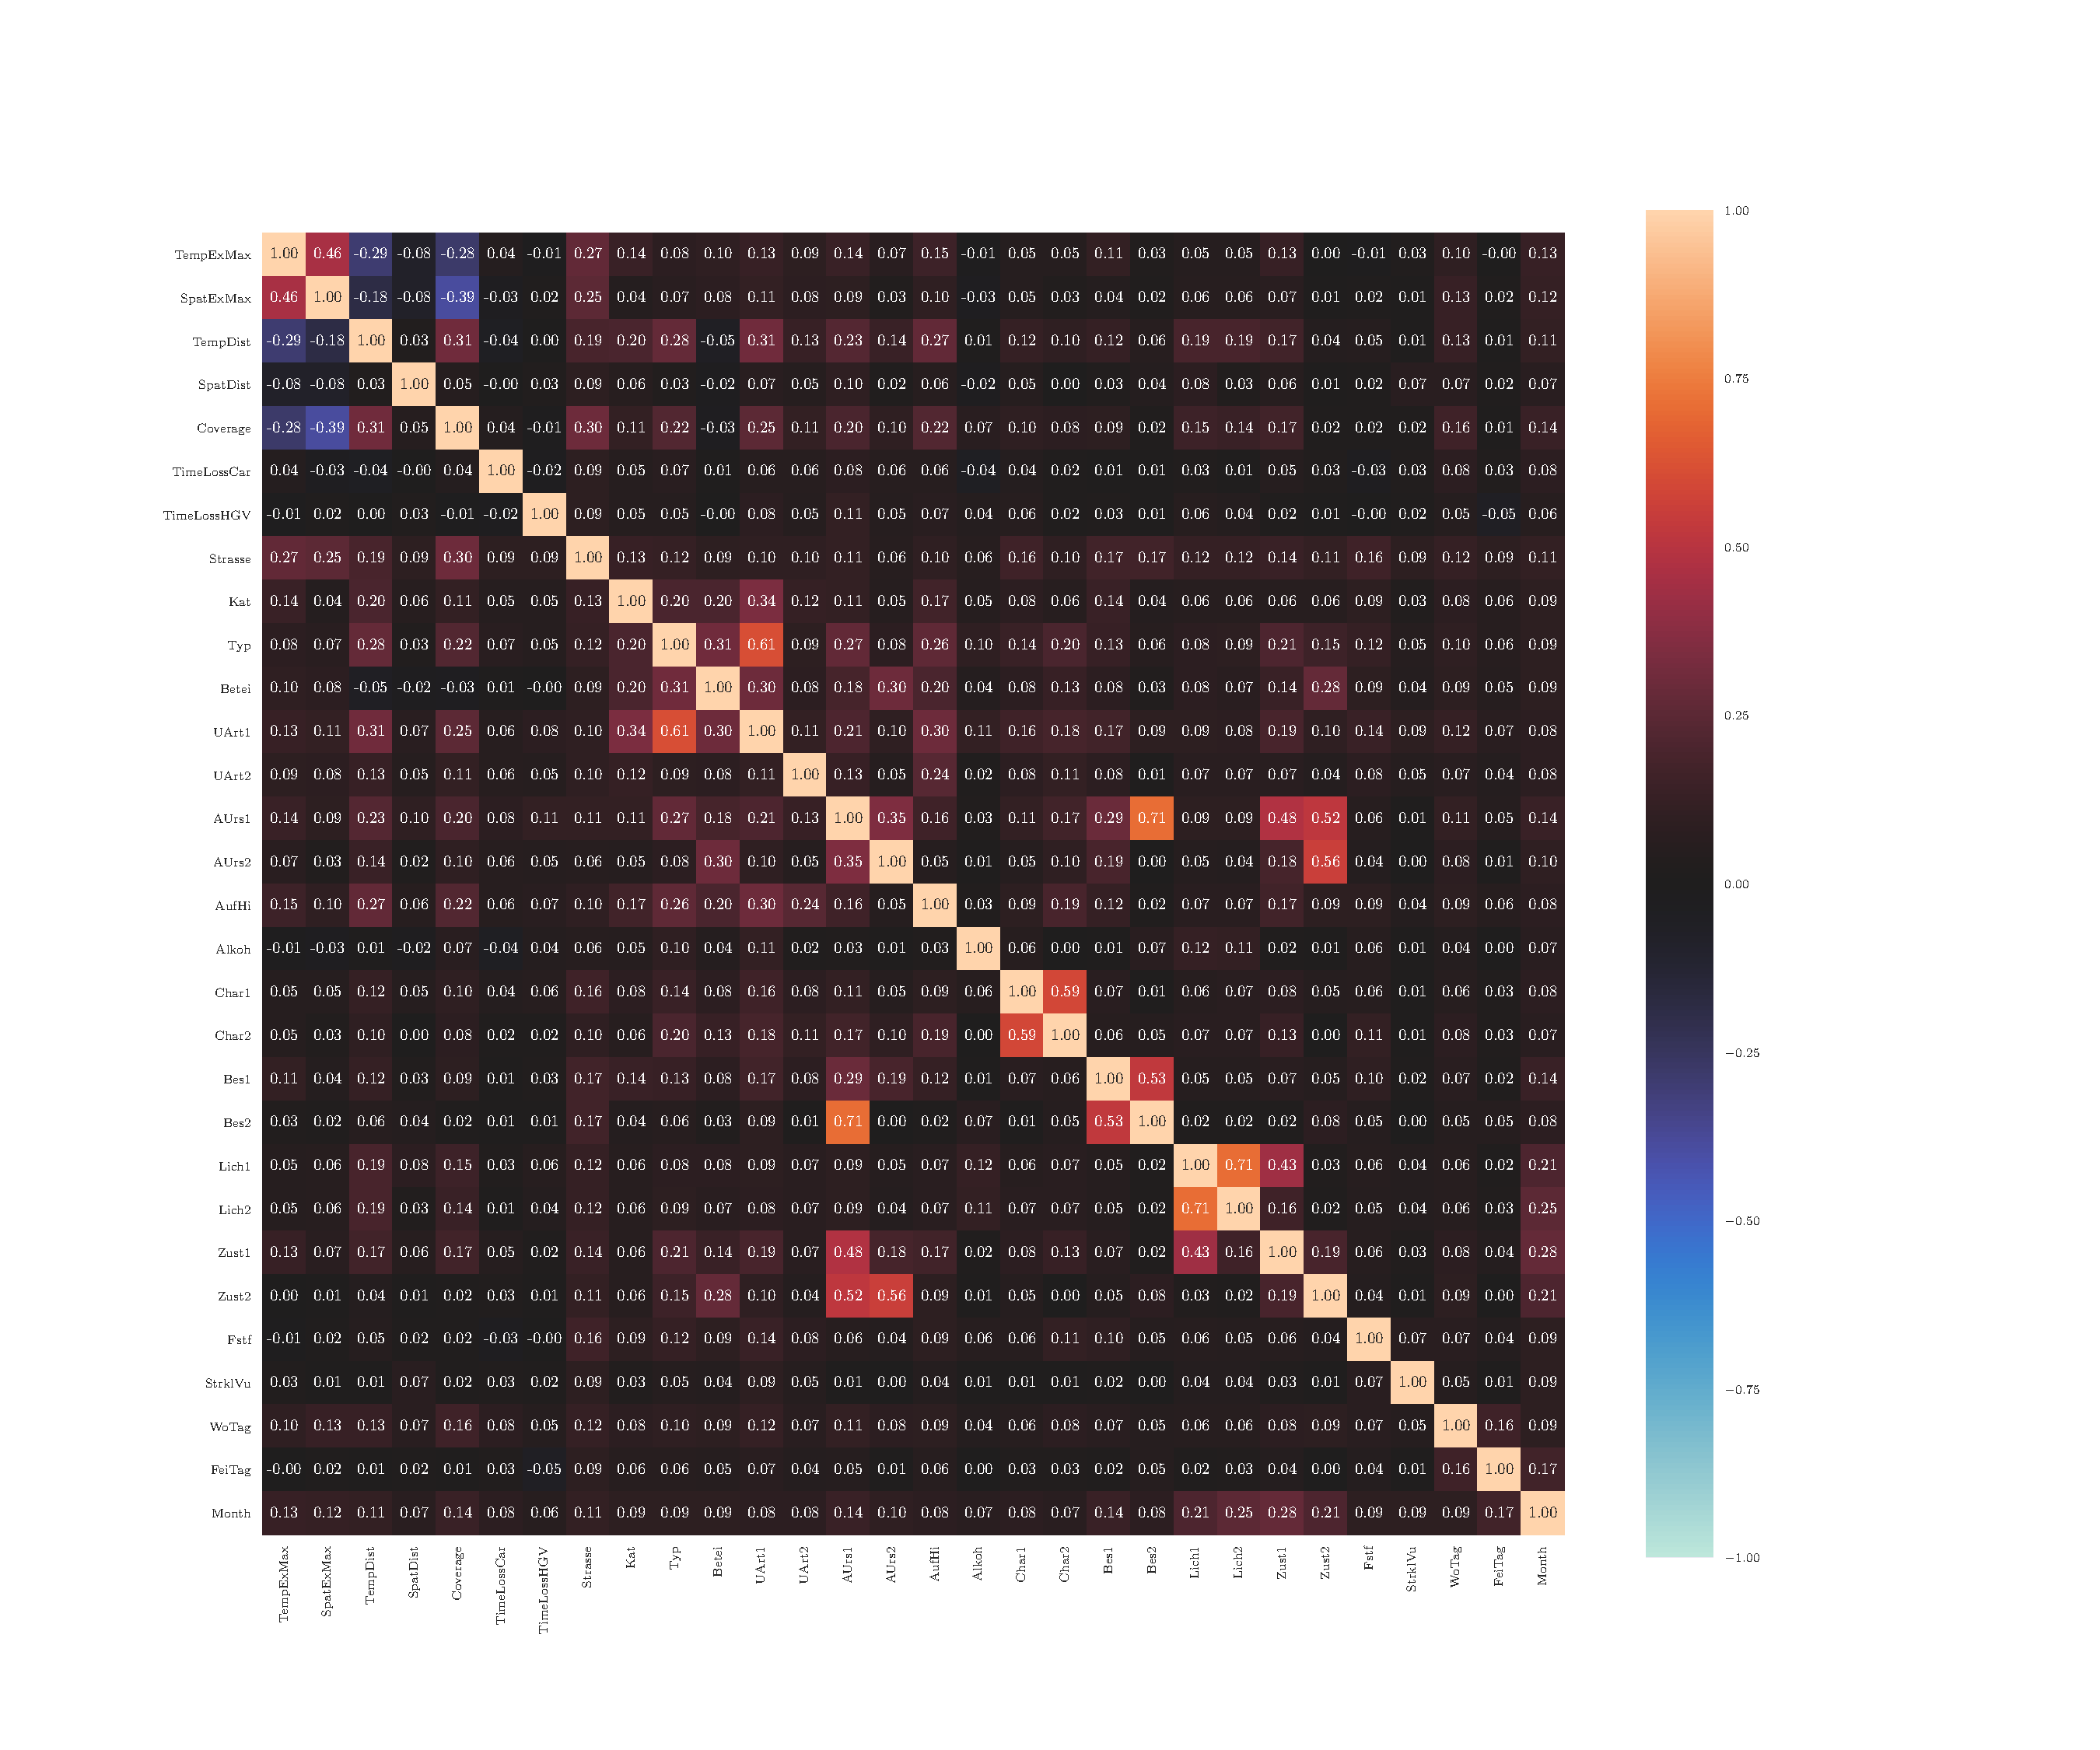
\includegraphics[scale=0.52, trim=3cm 2cm 0cm 0cm]{../CorrAnalysis/data/BAYSIS/02_matched/plots/baysis_matched_corr_cramers}
% 		\caption{Correlation matrix for BAYSIS matched data, with $V$, $\eta$, $\tau$, $r_{pq}$, $r$}
% 		\label{img:correlation_matrix_matched_cramers}
% 	\end{figure}
% \restoregeometry
\begin{figure}[!ht]
	\centering
	\makebox[\textwidth][c]{%
		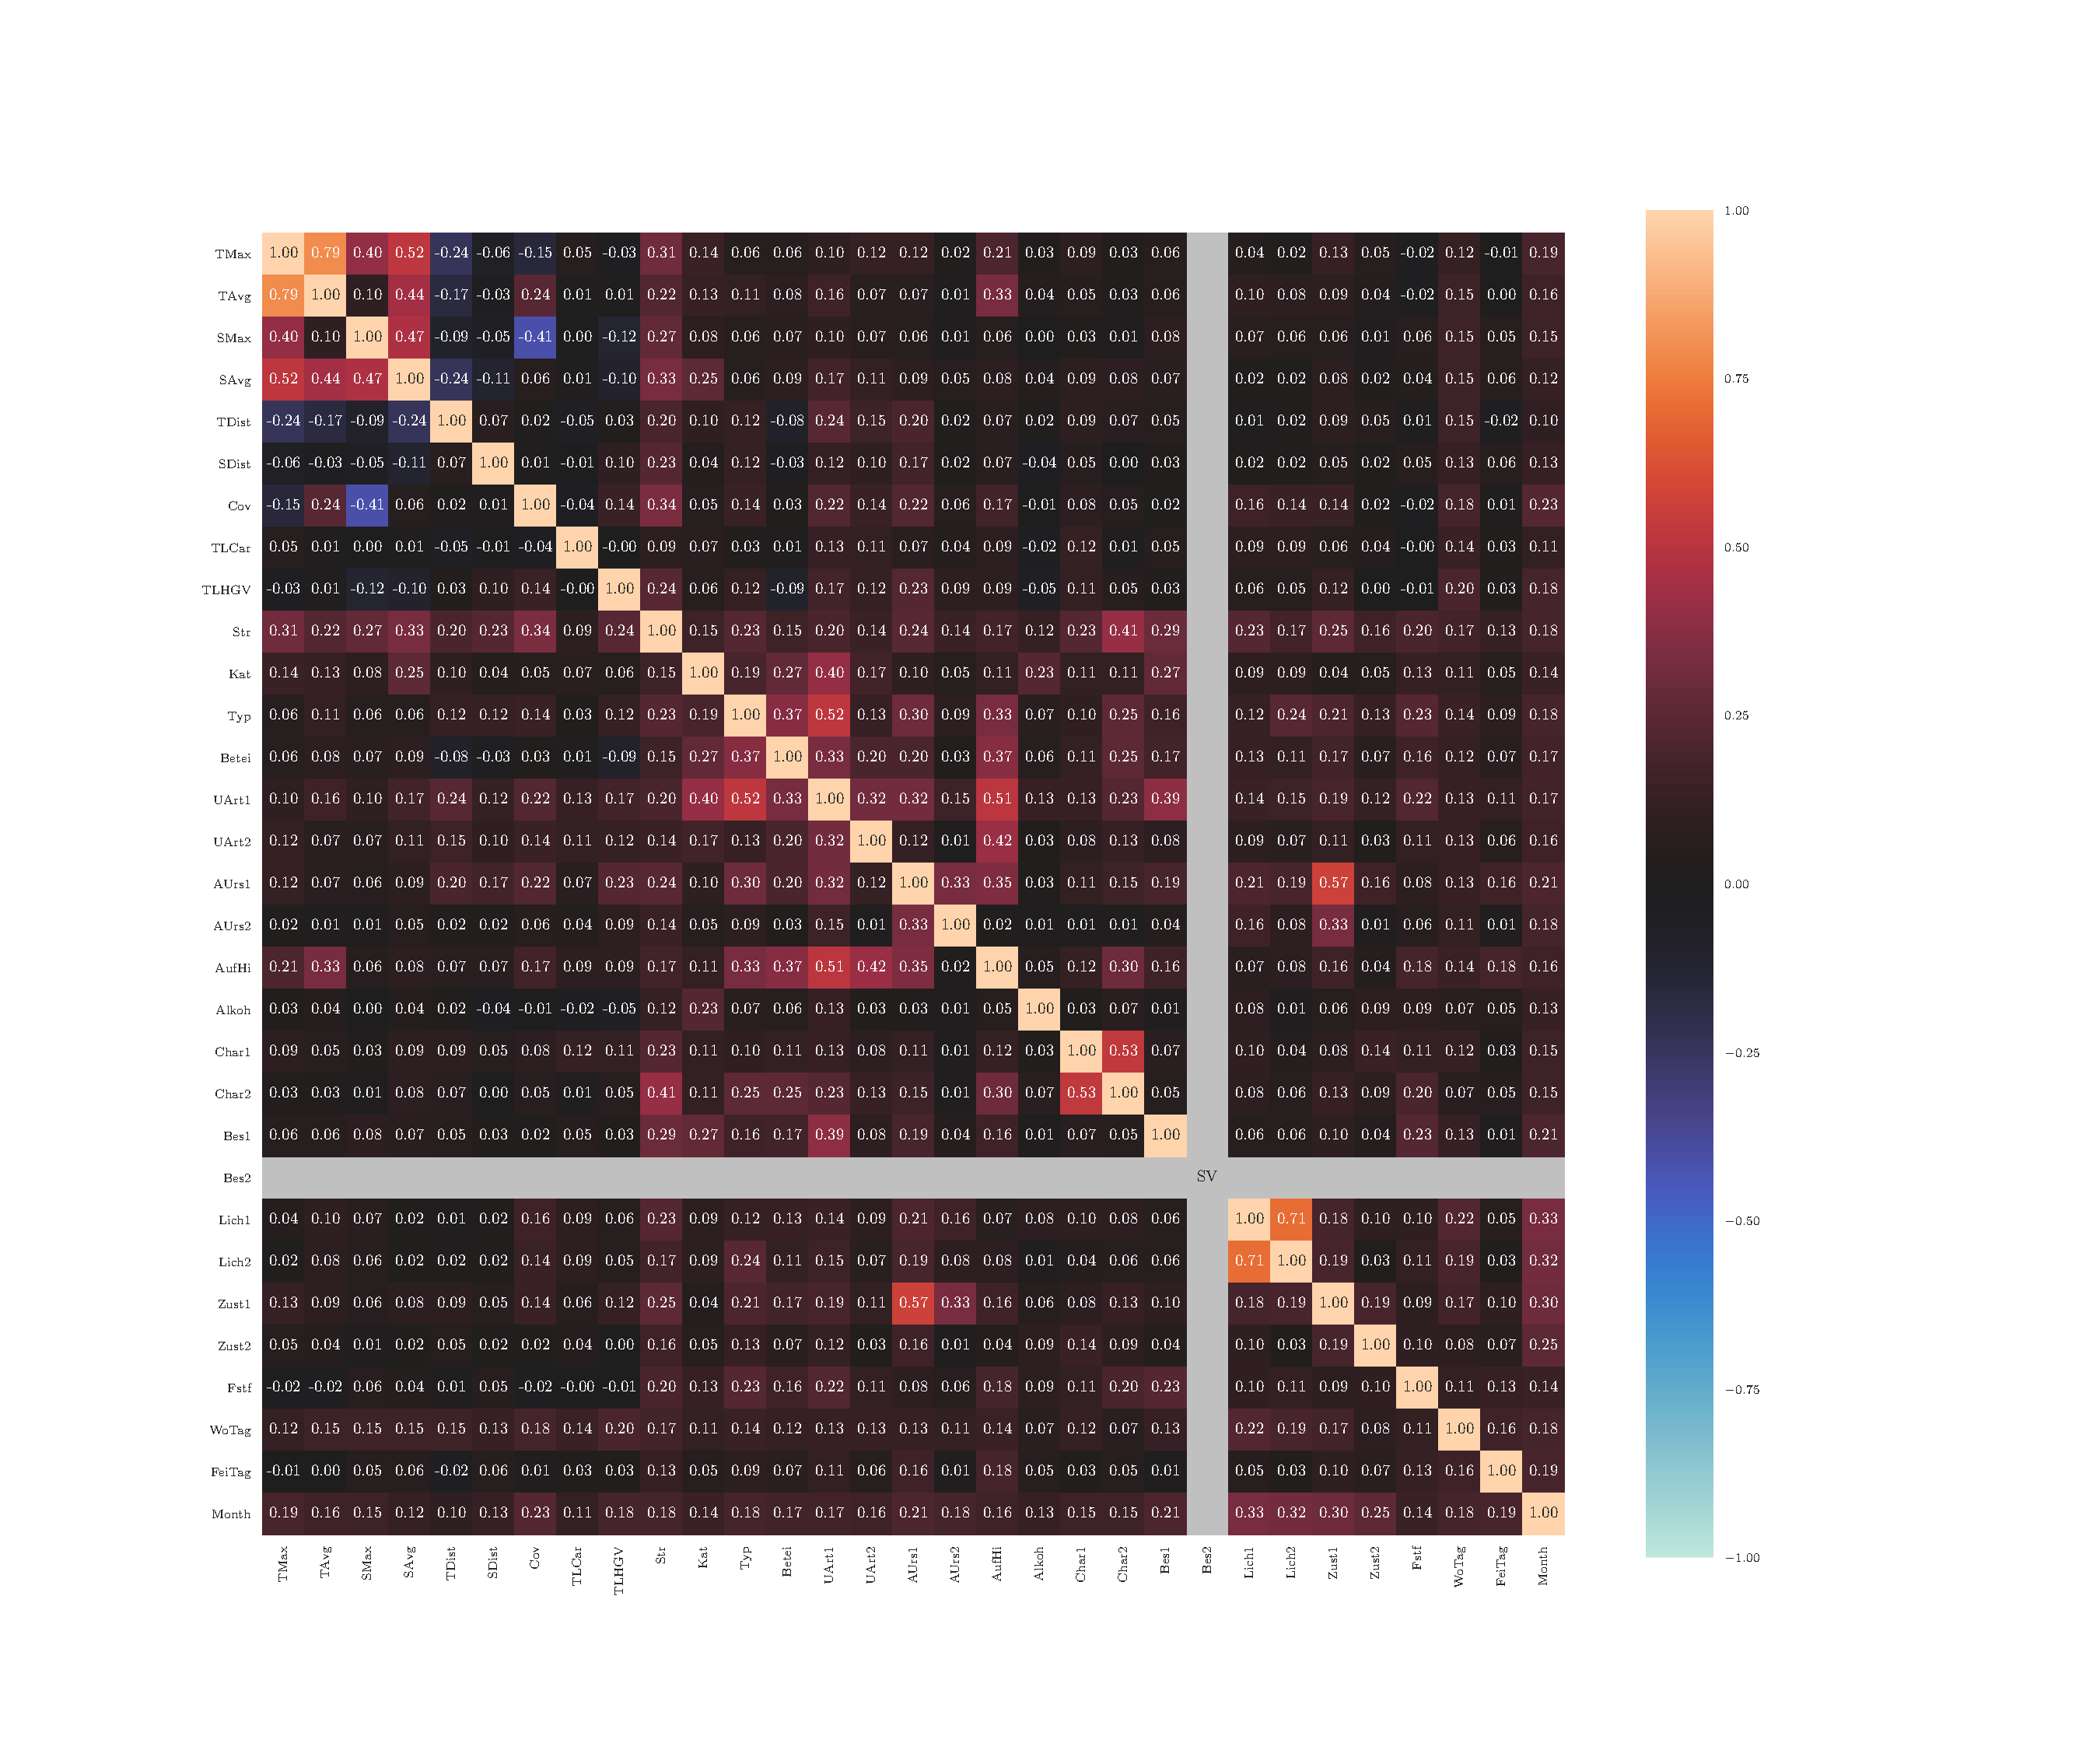
\includegraphics[width=1.4\textwidth, trim=0cm 2.5cm 6cm 3cm]{CorrAnalysis/data/BAYSIS/03_selected_03_endJam/plots/baysis_selected_corr_cramers}%
	}
	\caption{Correlation matrix for congestion-accident matched data classified as \textit{Jam Effector}, with $V$, $\eta$, $\tau$, $r_{pq}$, $r$}
	\label{img:correlation_matrix_matched_cramers}
\end{figure}

\large
\centerline{\textbf{Strasse}}
\normalsize

\paragraph{Maximal temporal Extent:}
\paragraph{Average temporal Extent:}
\paragraph{Maximal spatial Extent:}
\paragraph{Average spatial Extent:}
\paragraph{Temporal Distance}
\paragraph{Spatial Distance}
\paragraph{Coverage}
\paragraph{Time-loss HGV}

\large
\centerline{\textbf{Kat}}
\normalsize

\paragraph{Maximal temporal Extent:}
\paragraph{Average spatial Extent:}

\large
\centerline{\textbf{UArt1}}
\normalsize

\paragraph{Average temporal Extent:}
\paragraph{Average spatial Extent:}
\paragraph{Temporal Distance}
\paragraph{Coverage}
\paragraph{Time-loss HGV}

\large
\centerline{\textbf{UArt2}}
\normalsize

\paragraph{Temporal Distance}

\large
\centerline{\textbf{AUrs1}}
\normalsize

\paragraph{Temporal Distance}
\paragraph{Spatial Distance}
\paragraph{Coverage}
\paragraph{Time-loss HGV}

\large
\centerline{\textbf{AufHi}}
\normalsize

\paragraph{Maximal temporal Extent:}
\paragraph{Average temporal Extent:}
\paragraph{Coverage}

\large
\centerline{\textbf{Lich1}}
\normalsize

\paragraph{Coverage}

\large
\centerline{\textbf{WoTag}}
\normalsize

\paragraph{Maximal temporal Extent:}
\paragraph{Maximal spatial Extent:}
\paragraph{Average spatial Extent:}
\paragraph{Temporal Distance}
\paragraph{Spatial Distance}
\paragraph{Coverage}
\paragraph{Time-loss HGV}

\large
\centerline{\textbf{Month}}
\normalsize

\paragraph{Maximal temporal Extent:}
\paragraph{Average temporal Extent:}
\paragraph{Maximal spatial Extent:}
\paragraph{Coverage}
\paragraph{Time-loss HGV}

\subsection{ArbIS}

Analysis of the resulting separate datasets of congestion and incidents. What characteristic and key indicators are prominent?

What find of values, features and so on, does the dataset contain?

What time frame does the dataset cover and over what spatial area.

What kind of information does the dataset contain?

\noindent
\begin{table}[h!]
	\centering
	\begin{tabular}{c|l|l}  
		Category & Strong & Moderate \\
		\\[-1em]
		\hline
		\\[-1em]
		Strasse & TMax, TAvg, SMax, SAvg, TDist, SDist, Cov, TLCar, TLHGV & \\ 
 		%AnzGesperrtFs & & \\ 
 		%Einzug & & \\
 		%Richtung & & \\
 		%Length & & \\
 		%Duration & & \\
 		Month & TAvg, SMax, SAvg, TDist, SDist, Cov, TLCar & \\
	\end{tabular}
	\caption{List of incident variables and their strong/moderated correlated jam variable from the ArbIS matched data}
\end{table}

Are these correlations significant or not ? --> Wilcoxon Test

\paragraph{Strasse}

\paragraph{Maximal temporal Extent:}
\paragraph{Average temporal Extent:}
\paragraph{Maximal spatial Extent:}
\paragraph{Average spatial Extent:}
\paragraph{Temporal Distance}
\paragraph{Spatial Distance}
\paragraph{Coverage}
\paragraph{Time-loss HGV}

\paragraph{Month}

\paragraph{Maximal temporal Extent:}
\paragraph{Average temporal Extent:}
\paragraph{Maximal spatial Extent:}
\paragraph{Average spatial Extent:}
\paragraph{Temporal Distance}
\paragraph{Spatial Distance}
\paragraph{Coverage}
\paragraph{Time-loss HGV}